%%%%%%%%%%%%%%%%%%%%%%%%%%%%%%%%%%%%%%%%%%%%%%%%%%%%%%%%%%%%%%%%%%%%%%%%
%%%
%%% File: utthesis2.doc, version 2.0jab, February 2002
%%%
%%% Based on: utthesis.doc, version 2.0, January 1995
%%% =============================================
%%% Copyright (c) 1995 by Dinesh Das.  All rights reserved.
%%% This file is free and can be modified or distributed as long as
%%% you meet the following conditions:
%%%
%%% (1) This copyright notice is kept intact on all modified copies.
%%% (2) If you modify this file, you MUST NOT use the original file name.
%%%
%%% This file contains a template that can be used with the package
%%% utthesis.sty and LaTeX2e to produce a thesis that meets the requirements
%%% of the Graduate School of The University of Texas at Austin.
%%%
%%% All of the commands defined by utthesis.sty have default values (see
%%% the file utthesis.sty for these values).  Thus, theoretically, you
%%% don't need to define values for any of them; you can run this file
%%% through LaTeX2e and produce an acceptable thesis, without any text.
%%% However, you probably want to set at least some of the macros (like
%%% \thesisauthor).  In that case, replace "..." with appropriate values,
%%% and uncomment the line (by removing the leading %'s).
%%%
%%%%%%%%%%%%%%%%%%%%%%%%%%%%%%%%%%%%%%%%%%%%%%%%%%%%%%%%%%%%%%%%%%%%%%%

\documentclass[a4paper, 12pt, oneside]{report}    	%% LaTeX2e document.
\usepackage {tcdthesis}              				%% Preamble.
\usepackage{graphicx,color}
\usepackage{anysize}
\usepackage{amsmath}
\usepackage{pgfplots}
\pgfplotsset{compat=1.8}
\usepackage{lmodern}
\usepackage{url}

%\hyphenation{human, measuring, several, students}

\leftchapter                       								%% Uncomment one of these if you want  
%\centerchapter                      							%% left-justified, centered or
% \rightchapter                     							%% right-justified chapter headings.
                                     								%% Chapter headings includes the
                                     								%% Contents, Acknowledgments, Lists
                                     								%% of Tables and Figures and the Vita.
                                     								%% The default is \centerchapter.

% \singlespace                       							%% Uncomment one of these if you want
% \oneandhalfspace                   						%% single-spacing, space-and-a-half
 \doublespace                       							%% or double-spacing; the default is
                                     								%% \oneandhalfspace, which is the
                                     								%% minimum spacing accepted by the
                                     								%% Graduate School.

\renewcommand{\thesisauthor}{Michael Christian Frick}        	%% Your official UT name.
\renewcommand{\thesismonth}{September}             			%% Your month of graduation.
\renewcommand{\thesisyear}{2016}                     			%% Your year of graduation.
\renewcommand{\thesistitle}{\large{Learning Processes and Consistency in the Quality of Software Development Based on Environmental Influences} }            %% The title of your thesis; use mixed-case.
\renewcommand{\thesisauthorpreviousdegrees}{M.Sc.}  		%% Your previous degrees, abbreviated; separate multiple degrees by commas.
\renewcommand{\thesissupervisor}{Stephen Barrett}      		%% Your thesis supervisor; use mixed-case and don't use any titles or degrees.

	
\renewcommand{\thesisauthoraddress}{Dublin, Ireland}

%\renewcommand{\thesisdedication}{...}     %% Your dedication, if you have one; use "\\" for linebreaks.


%%%%%%%%%%%%%%%%%%%%%%%%%%%%%%%%%%%%%%%
%%% The following commands are all optional, but useful if your requirements
%%% are different from the default values in utthesis.sty.  To use them,
%%% simply uncomment (remove the leading %) the line(s).

% \renewcommand{\thesiscommitteesize}{...}
                                     %% Uncomment this only if your thesis
                                     %% committee does NOT have 5 members
                                     %% for \phdthesis or 2 for \mastersthesis.
                                     %% Replace the "..." with the correct
                                     %% number of members.

\renewcommand{\thesisdegree}{Master of Science in Computer Science}  %% Uncomment this only if your thesis
                                     %% degree is NOT "DOCTOR OF PHILOSOPHY"
                                     %% for \phdthesis or "MASTER OF ARTS"
                                     %% for \mastersthesis.  Provide the
                                     %% correct FULL OFFICIAL name of
                                     %% the degree.

\renewcommand{\thesisdegreeabbreviation}{M.Sc.}
                                     %% Use this if you also use the above
                                     %% command; provide the OFFICIAL
                                     %% abbreviation of your thesis degree.

\renewcommand{\thesistype}{Dissertation}    %% Use this ONLY if your thesis type
                                     %% is NOT "Dissertation" for \phdthesis
                                     %% or "Thesis" for \mastersthesis.
                                     %% Provide the OFFICIAL type of the
                                     %% thesis; use mixed-case.

% \renewcommand{\thesistypist}{...}  %% Use this to specify the name of
                                     %% the thesis typist if it is anything
                                     %% other than "the author".
                                     
%%%%%%%%%%%%%%%%%%%%%%%%%%%%%%%%%%%%%%%%%%%%%%%%%%%%%%%%%%%%%%%%%%%%%%%


\begin{document}                                  	%% BEGIN THE DOCUMENT

\thesistitlepage                                  		%% Generate the title page.

\thesisdeclarationpage									%% Generate the declaration page.

\thesispermissionpage									 %% Generate the copyright permission page

%\thesisdedicationpage                             %% Generate the dedication page.

\begin{thesisacknowledgments}                 %% Use this to write your
			                          							%% acknowledgments; it can be anything
Give many thanks and stuff...

\end{thesisacknowledgments}                    %% allowed in LaTeX2e par-mode.

\begin{thesisabstract}

The abstract or summary or whatever...

\end{thesisabstract}

\tableofcontents                                  	%% Generate table of contents.
\listoftables                                     		%% Uncomment this to generate list of tables.
\listoffigures                                    		%% Uncomment this to generate list of figures.

%%
%% Include thesis chapters here...
%%

\chapter{Introduction}

\begin{quote}
\centering 
\em % optional -- to switch to emphasis (italics) mode
"Be a yardstick of quality. Some people aren't used to an environment where excellence is expected."

\medskip
\raggedleft
Steve Jobs
\end{quote}
\vspace{10 mm}

Over the last years, the performance of computers rapidly increased and with it the complexity of the Software \cite{wirth2008brief}.
It can be a simple tool that is written in a short time by a single person or it can be a gigantic software project with several hundred developers involved in it\cite{cusumano1997microsoft}.\\
Different layers of abstraction from low level to high level programming languages actually make it possible to reduce the complexity of software projects. On top of that, there are libraries and frameworks that provide features that already have been implemented \cite{Martin:2008:CCH:1388398}.
An encapsulation of the modules is mandatory in order to allow splitting the work in a software project. A general structure must be given to ensure that the different parts can integrate easily and to keep the code understandable.\\
The more people work on one project, the more important it is to provide an organized and well planned architecture to keep the code clean.
\bigbreak
In today's world, software is everywhere! The traffic is controlled by computers as well as security systems, nuclear power plants or just a messenger app on a mobile phone etc. \\
The ubiquity of computers can make life easier, but can also cause unpredictable trouble.\\
In the early 1890s at the United Kingdom's Royal Air Force, an engineer found a bug that could have fired a missile without any command. Luckily it was found before a disaster happened \cite{ross2005exterminators}.
\bigbreak
The quality requirements vary for different software products. A crashing weather app on a mobile is not as bad as a bug that is causing a production stop in a plant. 
However, the quality of the software can make the difference whether a company will be successful or just be one of many abortive start-ups with a good idea but a bad execution.
\\
In the software industry, the most significant factor in the creating process is the human. The quality strongly depends on the performance of the programmers as a single person or in a team. That performance quality can change by various different reasons even a few times a day.
\bigbreak 
Previous researchers already did a lot of work in the field. \\
This dissertation will start with an overview of their findings which will include previous studies that investigated different theories about influencing factors on cognitive performance and related work.

\bigbreak
This dissertation describes a new approach where sensors and information from mobile phones were used to find evidence in factors that influence the performance of developers. 
We developed an Android application which was installed on the participants mobile device for the experiments. The app is gathering the location of the user, collecting sensor data from the light sensor, accelerometer, the environmental noise from the microphone and the data from the step counter of the device. \bigbreak

Two experiments investigated patterns in behavior and environment that are influencing the cognitive quality of a programmer. \\
In the first experiment, the mobile application gathered the data while the participant is solving a provided programming task and afterwards answering additional questions. \\
In a second experiment, only  the cognitive performance of one participant but in a more controlled environment was investigated. 

The first experiment investigated correlations of written code and data which was gathered during the development. The results have shown that more participants are necessary in order to find specific influencing factors. 

The individual experiment with the single participant provided evidence about influences of different music genres. Both resulting performances were also compared to a control scenario with no music played. The results for the participants arose that classical music reached the best results compared to heavy metal and the absence of music.\\
Also caffeine seemed to reduce the cognitive performance of the participant while, on the other hand running before solving the task showed evidence of a positive effect.
The results from the experiment with a group of participants shows no distinct patterns but traces of correlations between strong changes in the environment and distraction of the participant.  

\bigbreak
In the future, monitoring of developers performance could become ubiquitous in the industry and students. It could be used conjointly with project-management tools that track the development time on a specific project. It could simultaneously provide real time feedback about the code quality itself or divergent aspects in the working place and work patterns. Rather than only comparing the information with other app users, the app could also systematically develop an optimal working environment and behavior of the specific programmer.

\section{Motivation}
This section will describe the factor that motivated the topic of this dissertation and some background information. 

\subsection{Mobile Device Sensors}
Over the last decades the evolution of mobile devices began with a wireless telephone far away from pocket size. Over the years, the mobile devices got displays, SMS, telephone books, games and a lot more. In 2007, Steve Jobs introduced the first iPhone and with it the age of the smartphone  \cite{laugesen2010factors}. Over the years, smart-phones became powerful computers with a better display resolution than the most televisions and the computing power of what desktop pc users could just dream about a few years ago. More and more sensors were packet into the small handy devices.\\
The range of sensors reaches from proximity detection over accelerometer to humidity sensors etc. Google even engineered a system for 3D objects and indoor environments with just a single device in real time \cite{schops20153d}.\\
Thus, a lot of people own the hardware with the capability to collect rich context information and they even carry it with them all the time and has a lot of potential to support and improve the people's work and environment.

\subsection{Learning to write code}
Learning to write code is getting more and more important but still not a required subject in school. It is the software that is controlling almost everything in our everyday life such as traffic, gates, calendars etc. It's failure could have dramatic impacts in peoples life.\\
Thus, it is very important that programmers produce high quality code and also be able to find good frameworks and libraries. The problem is that it is not always obvious what high quality means. It can vary from good structured code to resource-aware, reliability and much more.
\\Still, many programmers didn't learn coding in school or university. They taught it to themselves and might just have used it for fun-project which were not created for public usage. However, they might not really know about best practices in the industry or how good or bad his/her code really is.\\
I experienced this problem myself.
When I started my first job as an iOS developer, I had no practical experience in writing code mobile applications. I had to maintain the current code and add new features in a big and unknown project. As I had no mentor or anyone who could give me feedback, I just did it as good as I could. I still don't know whether I created good or bad code. With a feedback tool for my code quality I could have learned a lot about the coding itself and by consequence, I would probably write much better code.

\subsection{The importance of Software Metrics}
Software is becoming more complex than ever and used in almost every environment. The deadlines in professional software projects are very strict and there is no time to develop everything from scratch. Development teams depend on libraries rather than reinventing the wheel over and over again. \\
As already mentioned in the previous section, a lot of people do programming for a hobby where the quality and performance doesn't matter to them as much as in a professional environment. They also create libraries and frameworks with their quality standards. The increasing amount of open source libraries and dependencies make it very hard, but also very important to professional developers to be able to trust the quality and functionality. At this point of time, the only indicators are user ratings and the amount of times it's been used in different frameworks and projects. Some few frameworks are also recommended in public reviews articles. \\
Frameworks and libraries also need to be dynamic and maintained. Operating systems and programming languages are being updated more frequently which requires fast changes. A constant measuring of quality at the first place could give direct feedback that the quality stays constant after changes and as well helps the developer to create a better structure and code to improve the maintainability from the beginning. \\
The most used platform in the open source community is Github. Github is based on git and is a web server that can be used to host software projects and allow to make them accessible to others developers  \cite{dabbish2012social}.

\subsection{Working environment}
A new trend, especially in the tech industry shows that company move from common clean looking office spaces to colorful creative environments. Companies like Google or Facebook seem to reduce the strict separation of work and personal life. Companies introduce unlimited holiday policies, provide free food and even have a laundry service for their employees. They try to remove all the obstacles from their employees life to allow them focus on their work.\\
Also the social aspect at work changes a lot. Some years ago, having a beer with the co-workers after office hours or meeting the colleagues for a ping-pong match during the day was unthinkable.\\
Google tries to motivate developers to communicate more with the team by placing the whole team in relatively small spaces and provide separate areas for tasks that require more silence. 
All these efforts to make the employees more productive are very interesting approaches but hard to measure. 
\bigbreak
In this dissertation, we are trying to find patterns between working environment, behaviors and the resulting code quality in learning and professional environments. Also, the creation of awareness for code quality and performance is an essential factor in the evolution of a programmer and is important at any stage of the experience. 

\section{Aims}
The goal is create a solid base and a working demonstration of a system that can gather data from a mobile device and show the significance of influences the quality in software development. 
This work and framework hopefully inspires and helps others to do more work in this area to bring code quality to a higher standard. 
Also for academia, a tool that provides feedback on code quality for the students can help to bring them on a higher level when they leave college. 

\section{Road-map}
The next chapter summarizes the related work in the area of software metrics, measurements and analysis, data gathering, data clustering, influences in cognitive performance and software quality.\\
Ensuing, we describe the design of the different software components to gather the data, provide information to the participants and to ensure the privacy of the gathered information.\\
Chapter 4 contains information and the process of the implementation of the different software components. 
The experiment is being described in chapter 5 and includes the setup and execution, the expected results. the next chapter characterizes data classification as well as the questions that are being asked to the participants. \\
The last two chapters describe and interpret the results and conclude the subject and information of the experiment.
The appendix contains an overview of the abbreviations, links to the source code and more details about results of the experiments.

                                
\chapter{The State of the Art}

\begin{flushleft}
Many researchers are concerned about finding metrics of software quality with the human factor as the most significant part in the development process. Research has also been done in the process of finding and testing factors which are influencing the cognitive performance of software developers.\\
In my dissertation I aim to identify environmental influences that can improve, worsen or influence the code quality of Computer Science students and professional software developers.
With the students as a key factor in future software engineering, I will analyze their behavior and performance influences in a environmental and psychological sense but also compare it with the numbers from the professionals. \cite{denissen2008effects}
\bigbreak
Measuring quality of software projects and gaining information about the progress are valuable information for the software engineers and developers to reflect their performance. The provided feedback helps them to identify their weaknesses and improve their skills or optimize their work patterns \cite{johnson1999leap} \cite{Martin:2008:CCH:1388398}.\\
Also project managers have a great interest in details about the progress and the products quality in order to coordinate the schedules, resources and have an overview about the possible bottlenecks in the project.
Early knowledge about potential problems can help them to target it and make a difference between the success or failure of a software project.
\bigbreak
A good programmer nowadays is described as a person who can solve complicated problems by breaking them down in smaller targeted problems that are easy to understand and to solve. Good code is supposed to be clean, easy to read and as simplyfied as possible \cite{johnson1999leap}.
\\
This new approach differs from the early days when programmers tried to find the shortest and most performant solutions. As long as code was using minimal resources it was fine. Less people were working on projects and the open source community was not as important and big as today and withe a lower computing power, the computers where unable to handle the complexity that software has today. 
More people are working together on different parts of complex systems. At the end every part must go hand in hand with all other parts and the code should have a similar structure so that people from one team could possibly also work or help out in another team.
\bigbreak
From a research perspective it is very interesting to get an overview approaches from different years to gain a broader understanding. Thus the following paragraphs will summarize information about code metrics and code quality from several decades.
\end{flushleft}

\section{Software Metrics}
Since the late 1960s, when the software engineering was in it's beginning, people wanted to measure and produce numbers to characterize code properties. 
The first metrics where used and developed to measure and evaluate the performance of a programmer. Lines of Code (LOC) per month and bugs per thousand lines of code (KLOC) are a very simple but efficient ways for examining the productivity, which can be used to for comparison with other programmers or general standards.
\bigbreak
Software metrics is the term that is been used more then 30 years ago up to today.
Today, some of the most metrics are still being used to investigate the productivity of the software developers. The amount of bugs in relation to the amount of code, the initiall number of requierements compared to the requierememts at the current point in the project and the effort it takes to fix faults versus the total time the project reqieres. \cite{kaner2004software}
The metrics have been a great success in the industry. Most of the big software companies and even smaller ones use metrics, though they are barely used in academia. 
The metrics are created for larger software and scopes. Also maintenance and re-factoring is not as important in academia as it is in the industry with commercial software. Also, Software metrics in the industry are primarily important for the management rather than for the development process.\\
Industrial software metrics can be used to ensure quality, productivity and even for predictions of the software quality and it's reliability \cite{fenton1999software}.
Several researchers investigated and developed approaches to improve the metrics and the results which they are generating. 
Yue Jiang et. al. \cite{jiang2008comparing} from West Virginia University researched methods for improving software quality predictions. They used supervised machine learning algorithms with datasets and focused in improving of the information content of the training data in their research. The results at the end showed that the biggest differences in the quality of the predictions are generated by the choice of the right software metrics rather than applying different machine learning algorithm. 

\section{Metrics Measurement and Analysis}
PSP - Personal Software Process is a way to gather data about the Software engineering process and analysis of the information.
Over the last decades, the University of Hawaii did a lot of research about PSP and they developed different approaches to make students to adopt and use it in their project and even later at work.
Their first approach was originally described as ``A Discipline for Software Engineering''. It required the users to keep records about all the metrics by hand. The massive overhead was a high barrier for the students to adopt and keep on working with the PSP. For the best results they needed to write down every compiler error and they had to track the time they were working on their projects and had to stop it for interruptions.\\
In 1998 the University of Hawaii started the Leap research project to provide a PSP with low overhead for the collection and analysis of the data. This generation of PSP was using automated tools which were asking the user for inputting the data. These tools were also able to display information and analyses to the user.
Just a few students adopted the system. The researchers found out that another reason for the reluctant adoption was the constant context switches for the users. Inputting the data during the programming task interrupted and disturbed the ability to focus on the programming tasks. \cite{johnson2003beyond}
In order to eliminate the adopting barriers, they started the Hackystat project in 2001. Hackystat is an open source framework for automatically gathering all the required metrics by data collection plugins in the development environments of the users.\\
Plugins, that are installed by the in their programming environments automatically collect the data and forward it to a centralized web service. The web service orders and analyzes the data. If interesting results occur, the webservice sends emails to the developers to inform them about it. The web service also provides a rich visual representation of the data.
All the different approaches to provide feedback about the code lead to improvements in the quality and the ability to estimate software projects. \cite{johnson2001project} 
The Appalachian State University in North Carolina described a different approach. Their goal was to decrease the high attrition rate of computer science students and increase the attraction to get a computer science degree in general.\\
The researchers were monitoring the students software development behaviour in order to find good practises for successfully learning programming. For gathering the data of the individual students, they developed a tool called ClockIt. ClockIt allows to, fully automatically, collect the data, analyze it and compare the results with the results from better or more experienced students visually. A web interface provides access to measurements for the student, the course instructor or an administrator.\\
In their results they compared the data of three students out of 75 participants. The students with the best results, an average scoring student and the one with the lowest grade. 
The comparison showed that the best student also spent the most time on the project, but wrote less code than the average scoring student who spend almost as much time. The worst student spend the least time and submitted the smallest amount of code. There was an interesting correlation between the grade and the compilation errors and the amount of compilations that were made. The best student compiled the code more than double as much as the average student and almost 6 times more than the worst student did. \cite{norris2008clockit}

\section{Mobile Data Gathering}
Ferreira, D., et al. \cite{ferreira2015aware} from the University of Oulu, Finland and the Carnegie Mellon University were working on a toolkit for gathering the sensor data from mobile Android devices. They created an extensible framework that could have been used in any Android application at the time when the paper was released. They also released an application for research purposes (the Aware client). The Aware client is extendable with plugins to support more than the pre-installed sensors. By default, the application stores the gathered data on the local hard disk but can also be uploaded to a database.\\
The sensoring is optimized to keep the energy impact as little as possible and not to use more device resources than necessary.
\bigbreak
Another approach in the area of mobile data gathering have been made by University of Science and Technology of China HUI XIONG, Rutgers University in cooperation with Nokia. In order to detect the context of the mobile device, Zhu, Hengshu, et al. \cite{zhu2015mining} were reading the log files of the device. The device logs provide information about location, accelerometers and optical sensor as well as browser history or which apps were used and are automatically recorded by the Android operating system. These information can be used to provide context aware suggestions e.g. for other games or based on the physical location. To read the logged information, the needs to be physically connected computer.\\
The information from the device logs are much richer than the information which can be gathered in an application with the downside, that the device needs to be connected to a computer in order to access the information. A installed application can compute, store and transfer the data  to a remote server from everywhere. The only requirement is access to the internet. 

\section{Variable Quality Influences}
The whole software quality is based on the cognitive performance of the software developer and the communication within the team. 
When the single developers write brilliant code, but don't know what the others do or need, the code can't work. On the other hand will the code quality still bad when the development team communicates perfectly but the individual programmers write bad code \cite{moe2010teamwork}. The following sections will provide an overview about the previous research of the individual factors in that area. 

\section{Team Communication}
The differences between team with high cooperating teams against project team with less communication have been investigated an discussed by Mary Beth Pinto and Jeffrey K. Pinto \cite{pinto1990project}. They tested the two different groups on the task and the psychological outcomes. Several different factors have been tested significantly better in the high communicating group. They scored higher in resolving problems, brainstorming, progress review, obtaining information, gaining authorization to perform tasks and in receiving feedback. The low cooperating team did just get a better score in resolving conflicts which is not surprising as fewer communication creates less conflicts. 

The importance of the communication in software teams is gaining more and more attention from companies within the last few years. A term which is used a lot are agile software engineering methods. The concept is based on flexibility and responsibility. Instead of having a the whole project scheduled at the beginning, agile concepts allow to react to problems and new information in a faster way /cite{chow2008survey}. One of the most used and successful methods to work in agile teams is scrum.

In scrum, the tasks are separated in, so called sprints. A sprint is a short time period in that a defined goal should be reached. This goal can be for example a feature or a new component. After the sprint the team comes together again and decides about the next sprint. I this way the team has a lot of responsibility about the project and a lot of freedom how they reach their goals within the sprint period. At the end of a sprint or a defined period, the team comes together for a retrospective to discuss the last sprint/s and how to improve the processes in the next period and if they change some methods such as the daily meeting. Daily meeting is done buy some scrum teams, where every team member summarizes the achievements and problems from the previous day. This meeting can be useful or just wasting time. In Order to find the best working and management patterns the teams can test different methods and discuss them in the retrospective. This dynamic changing and regular feedback is one of the reasons why scrum is used more and more in modern software teams \cite{rising2000scrum} \cite{moe2010teamwork} even with problems like the increasing need to trust the emplyees and control for a company \cite{ramesh2006can}.
\bigbreak
Another problems with the communication in teams comes with the increasing globalization and the internet. The ability that and employee can work from every part of the world with an internet connection brings the disadvantages that the software developers don't sit in the same room anymore or are working within walking distance. Also homeoffice for a few days a week is an option that employers provide their employees in order to be a more attractice and family freindly company. These changes also requiere new techniques to communicate within the teams. Communication could be done by using video conferences or email. However, both techniques have their disadvantages that a videocall needs to be scheduled and requeres a good internet communication and the problem with emails are the delayed response times. \cite{carmel1999global}
A solution are chat programs that are finding their way more and more in the daily communication in software development teams \cite{jarvenpaa1998communication}. Slack is the most used tool for chatting at work and the Company the fastest growing Startup in the world. After just twenty month after its launch in February 2014, already more than 1.7 million people where using Slack  \cite{bercovici2015}.

\section{Cognitive Performance}

\subsection{Context Switching}
\cite{pope2015impact}

\subsection{Work environment}
Improving the perfomance in Software Development can be done in a several different ways. One approach to improve the performance is the optimization of the working environment. Amabile, Teresa M., et al. \cite{amabile1996assessing} wrote about a conceptual model for increasing creativity in the work environment. Five key factors were described. The first two factors were, the encouragement for innovation and creativity as part of the company culture as well as according autonomy or freedom for the employees. Another key described the adequate availability of resources for a project which might affect people psychologically by the feeling to work on a valuable project. Also pressure at work was identified to increase creativity on a balanced level between excessive demands and boring routine. The last key factor in their model described the organizational impediments to creativity which could be caused by internal competitions.
A study was designed to investigate two hypotheses: The influence of the model in high-creative projects vs low-creative projects is expected to be much bigger. As well as obstacles scales are lower in high-creative projects compared to low-creative projects for workload with pressure and organizational impediments.
Both hypotheses had clear result outcomes, which showed that beside the employee's itself, the management can significantly influence the level of creativity and innovation by forming the organization culture. The construction of the teams and definition of the individual roles can have a great impact on the creativity. 

\subsection{Arousal}
The cognitive performance can very based on the context and the environment. When the body is in a relaxed state, the mind also slows down to save resources. Back in the stone age that made sense because thinking was not as important as today. Cognitive performance was mainly needed in dangerous or unusual situations where the heart beats faster and provides the brain with more oxigen and the arousal is higher than normally.
Researchers from the Brunel University in the UK showed movie clips to invoke different defined moods of the participants before they solved given debugging/coding tests. The results showed improvements in the results after the participants were seeing high arousal video clips. Low arousal clips affected the performance negatively compared to neutral clips. \cite{khan2007mood}
It is called the Yerkes-Dodson Law, that proclaims that a higher level of arousal leads to better cognitive performance. As caffeine also influences the arousal, it also can boost the cognitive performance and is not just helping to wake up in the morning. Watters, Paul Andrew et. al. \cite{watters1997caffeine} found out that the mean for the best cognitive results is an amount of 400 mg caffeine (the amount contained in ca. 5 espresso shots).
\bigbreak
When an arousal is influencing the performance of a programmer other factors that are effecting the mood could also have an impact in the quality of the written software. Many people believe that, for example the weather has a strong influence in the daily mood of a person. Certainly, Denissen, Jaap JA, et al. \cite{denissen2008effects} found out that the sunshine alone actually has no noteable effect in the mood of the most of the people. However, they found significant correlations between sunlight, air pressure and precipitation on the tiredness of the participants.
A reason for the influence of sunlight could be vitamin D3. The most of it is obtained through exposure to sunlight and it changes the level of serotonin which was found to be partly responsible for the mood of a human.

\subsection{Diet}
A very different, but probably the most important factor in the long term cognitive performance is the consumed food. The human brain needs good fuel to run properly. A wrong diet can strongly influence the incidences of cognitive problems as well as healthy food can positively influence for healthy ageing \cite{spencer2008food}.\\
Some foods demonstrated positive effects on the mental performance containing flavonoids like for example grapes, tea, cocoa and blueberries. 
Different to the previous influences, the diet and the lifestyle are less obvious. Their impact is slowly showing over years and it's hard to prove their effects and that they are the influencing factors.\\
Studies on several mammalian species have shown that food which is rich of flavonoids have beneficial effects on memory and learning with the ability to support neurons and protecting them again stress-induced injury.
It also decreases the chances of alzheimer and dementias. Other studies have shown that flavonoid-rich food improves the blood circulation and correlates with the growing of new hippocampal cells. These cells are located in the brain region that is identified to be responsible for the memory.                                
\chapter{Design}

\begin{flushleft}
In this chapter, I describe the design of the Android application which is gathering the data. I will also outline the sever side implementation to compute, store and provide information. Afterwards follows a short description of some additional tools, needed for the data analysis.\\
First, I will start with a brief description of the two components and will follow with my design decisions and my reasons for the choices. 
\end{flushleft}

\section{Functionality Overview}
The purpose of the application is to gather information from a mobile device of a participant while he/she is working on a programming task. Afterwards the application sends the collected data to a server for further processing and analysis. The participant also simultaneously submits the written code which code quality will be detected and then correlated with the processed mobile device information. 

\section{Mobile Application Design}

% Define bar chart colors
\definecolor{others}{HTML}{e78d1c}
\definecolor{android}{HTML}{a4c639}
\definecolor{ios}{HTML}{1c90e7}

\begin{figure}
	\centering
	\begin{tikzpicture}
        \begin{axis}[
            width  = 0.85*\textwidth,
        	height = 8cm,
        	major x tick style = transparent,
        	ybar=2*\pgflinewidth,
        	bar width=30pt,
        	ymajorgrids = true,
        	ylabel = {Market Share (\%)},
        	symbolic x coords={4Q14, 4Q15},
       	 	xtick = data,
        	scaled y ticks = false,
        	enlarge x limits=0.25,
        	ymin=0,
        	legend cell align=left,
        	legend style={
                at={(1,1.05)},
                anchor=south east,
                column sep=1ex
        	}
      	]
     	\addplot[style={android,fill=android,mark=none}]
            coordinates {(4Q14, 76.0) (4Q15, 80.7)};

        \addplot[style={ios,fill=ios,mark=none}]
             coordinates {(4Q14, 20.4) (4Q15, 17.7)};

        \addplot[style={others,fill=others,mark=none}]
             coordinates {(4Q14, 3.7) (4Q15, 1.5)};

        \legend{Android, iOS, Others}

        \end{axis}
 	\end{tikzpicture}
 	\caption{Smartphone OS Marketshare}\label{result}
 	\vspace{10 mm}
\end{figure}

\begin{flushleft}
In quarter 4 of 2015 Android had a market share of 80.7\% in smart-phone sales by operating system (see Figure \ref{result}). The trend also shows that the number increased from the last year \cite{gartnerMobileOSMarketshare}. Therefore I decided to realize the mobile application implementation for Android in order to be able to work with more users who have access to that application.\\
An alternative to the native implementation (e.g. iOS or Android) could have been a hybrid application. A hybrid apps is based on web-technology and using the addvantage of resposive web design to be able to work with every aspect ratio and resolution on an mobile device. One way doing that would be by using a framework such as PhoneGap, wich internally creates a native webview applicationand just loads the hybrid JavaScript, HTML, CSS in it. Another software for cerating a hybrid solution is Titanum accelerator which itself is using native UI components. Both frameworks have the advantage is the simple development and the OS independence. The problem with hybrid apps are the performance and limited accessiblity to hardware components including some sensors \cite{holzinger2012making}.  
\bigbreak
The Android application make use of its build in sensors and information provided by the Android operating system \ref{sensors}. Different than iOS, Android is an OS that can be installed of different devices from different vendors and with different hardware components \cite{goadrich2011smart}. Thus the buit in sensors which are clustered in motion sensors, environmental sensors and position sensors \cite{androidDevelopers} can differ between the different devices. Components which are required for standard functionality such as making phone calls are more common than other sensors. For example the the microphone for recording the users voice or the light sensor, which is used to detect whether the user has the phone at his ear can be found in almost every mobile android device. 
\end{flushleft}

\begin{figure}
\centering
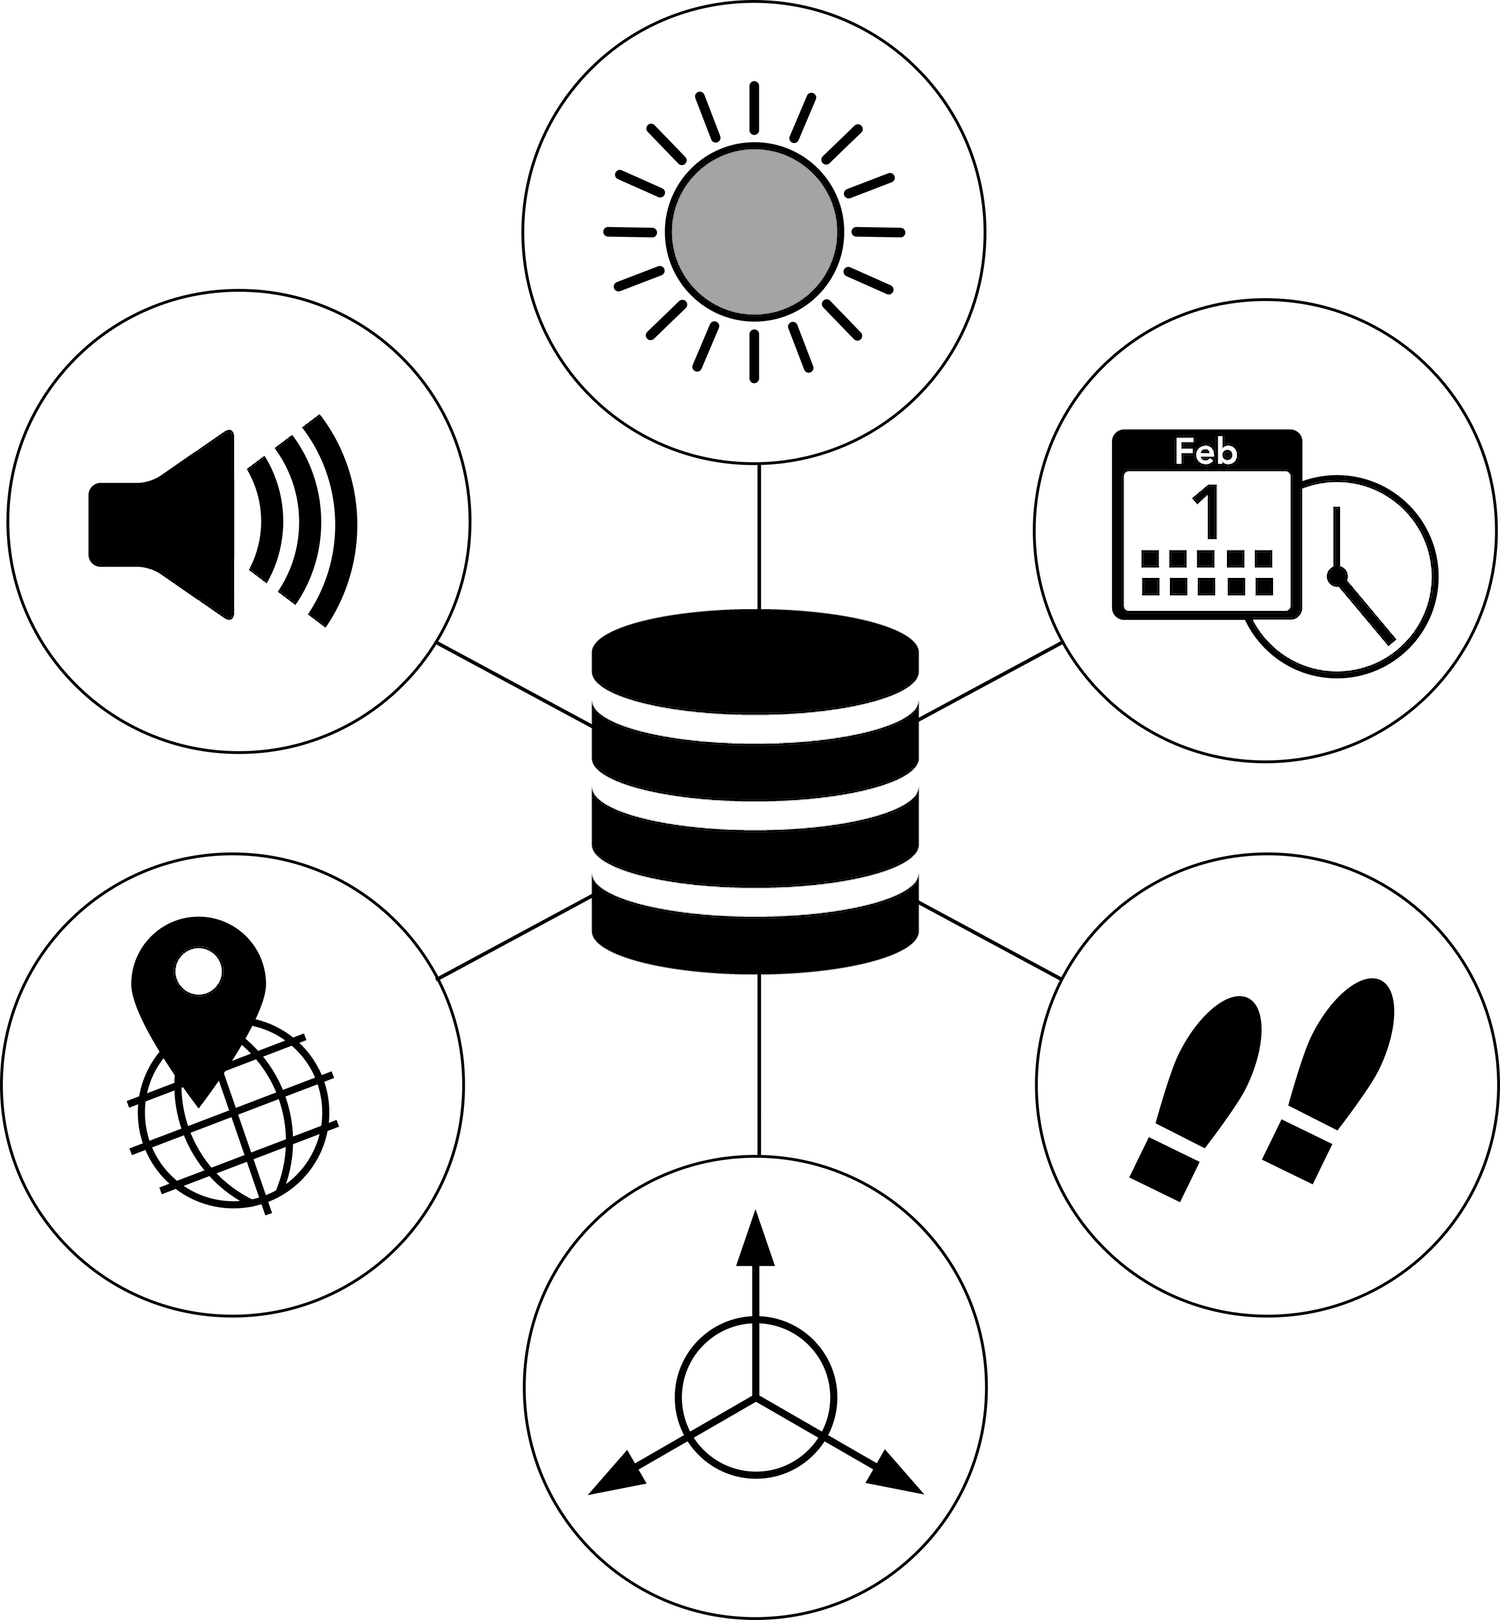
\includegraphics[width=8 cm]{sensors}
\caption{gather data: light, timestamp, steps, accelerometer, location, volume}\label{sensors}
\vspace{5 mm}
\end{figure}

\subsection{Requirements}
The application is primarily created for the research project and therefore not for the everyday use. The participants should not waste much time in finding out how the app works. The goal was to create a simple and intuitive interface and a leading flow trough the functionality. The apps purpose is to gather the data of the participant during coding. That includes the usage of the mobile device during work. Thus, the gathering app must be able to run in the background, so the participant can use the app as he/she would normally do (e.g. Listing to music, texting etc.)

\subsection{App Architecture}
The Android app is built based on the Model View Controller design principles. This design principle defines the interfaces between the three different parts, the Model, the View and the Controller and states the tasks and responsibilities of each part.\\
The Model is the data source and in this app represented by the SQLite Database and can only communication happens to the Controller. 
The Controllers are called Activities in the Android Framework and is responsible for managing the Views, which are defined in XML files and then modified by the responsible Controller. 
To keep the code base clean and to avoid bugs, the communication is separated by the controller. The Model doesn't directly communicate with the View and can't update it. It the case of changes, the Model informs the Controller, which decides whether or not to update the view etc. 

\subsection{User Interface}

\begin{figure}
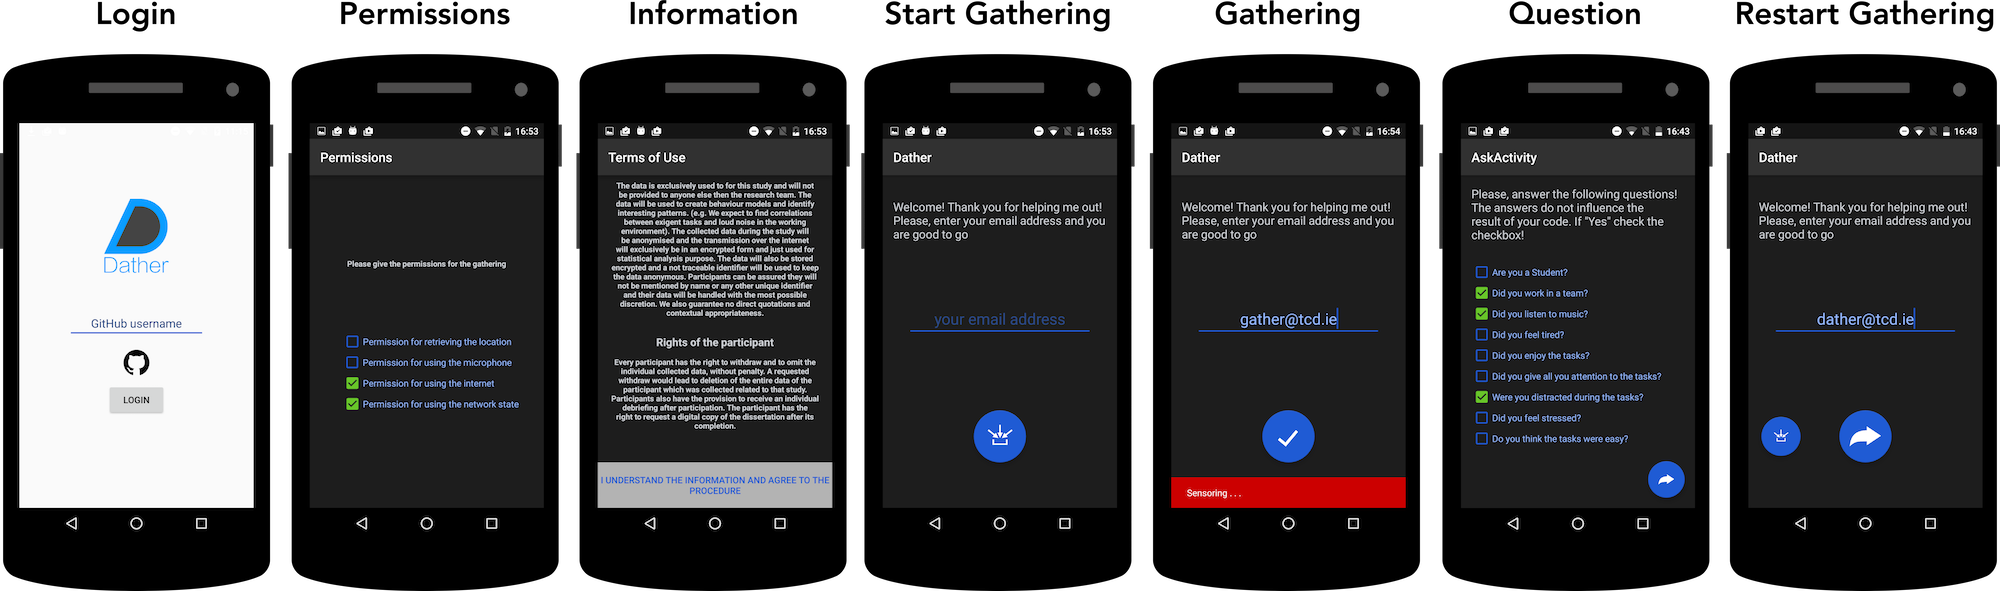
\includegraphics[width=\textwidth]{AndroidUI}
\caption{Android Views}\label{aviews}
\vspace{10 mm}
\end{figure}

The Application contains of two main user Interfaces, the gathering view and the question view.\\
The gathering view is the control interface for starting and stopping the data gathering. Its interface changes depending the current state and the logical functionality and also provides an input field for the users email address.
\bigbreak
After sending the gathered data to the server the application displays the question view. Here the user sees a number of questions and check-boxes to answer the binary yes and no questions. 
This interface also provides a send button to submit the answered questions to the Server.
\bigbreak
In Figure \ref{aviews} you can see the flow of the views in the applications.

\subsection{Data Storage}
For storing the gathered data entries, the app uses a SQLite datebase. SQLite uses SQL syntax which and is embedded in Android and well documented by Google. \cite{vogel2010android}. It is a very light weight database and provides an abstracted and easy way to store the values in an object oriented environment. SQLite is storing the data unencrypted by default. In order to make sure the stored data is save and can't be read, the data is been encrypted as soon it's been gathered.\\
The database has a capacity of 1024 MB which is equal to 1,000,000 KiB and can store 2,380,952 entries of an average of 0.42 KiB (this value is calculated based on the used storage of 1,000 entries). Assuming that the maximum gathering get 30 entries per minute, the database can store 7,9365.07 minutes or 1,322.75 hours of the gathered data. 
\\bigbreak
Additional to the SQLite database, Android provides a way to store single entries such as the field with the email address of the user. The so called "shared preferences" are storing key-value-pairs persistently on the phone and can be accessed from everywhere in the application.

\subsection{API}
The gathered data and afterwards the answered questions will asynchronously send to the Server and written into the database. When the response will be received, the view shows a visual confirmation and moves on to the next step or in case of the questions back to the gathering interface. 
\bigbreak
The communication to the Server uses HTTP connection over a stateless REST-full service. The REST-Service is a centralized way to allow making entries to the database and use the computing power of the server. PHP is the programming language used server-side and is establishing the connection to the MYSQL database.\\
As this application just requires to send information to the server but not receive information, the data gets converted to JSON format and send to the server via a POST request. The server response with a success or fail and provides some additional information in case entries were added to the database. 

\subsection{User Information}
For accessing the information from the mobile device, Android requires the user to granting the permissions for specific functionality such as using using the internet connection of the phone or access information like the telephone book entries.\\
The permissions were given when the the user by simply downloading the app from the PlayStore all in one place. However, since Android 6, the developer now is forced to ask for the permissions within the application itself  \cite{androidpermissions}.\\
Thus, the users with Android 6 or higher are provided by a additional interface which is specifically asking for permissions for Internet Access, access internet state information, using the device microphone and getting the location of the device. 
\bigbreak
Independent from the Android version the user needs to read and accept the terms of use at the first start of the application. The displayed text informs the user about the rights and what is happening with the data and information the user provides through this app usage.
\bigbreak
Within the app the user is asked to enter his/her email address. The email address then is being hashed with the SHA256 algorithm to ensure the data will be anonymous and can't connected to the user.   
\bigbreak
Also the gathered data are stored encrypted in the SQLite database on the mobile device and just decrypted on a local computer after the researchers downloaded the encrypted entries from the SQL database on the server. That ensure that the files are not accessible in readable format at any time. 

\section{Server Design}
The server is hosted by 1\&1 Internet SE as a completely pre-configured server backend PHP version 5.6 and the MYSQL-server phpMyAdmin in version 4.1.14.8. The also pre-configured server file system can be accessed using SSH or via FTP.

\subsection{requirements}
The Website is required to provide all the information a participant could need to do the experiment. The Interface should be clean and the participant should be also able to download the android application from the same website as he/she gets the information about the experiment. 
The backend will only be used by the researchers and therefore the user interface doesn't matter as much as for the participants. The functionality and the customization are the most important features. 

\subsection{Server Frontend Design}
The information for the participants of the study can access information web pages and access the downloadable Android application.\\
The frontend is implemented in HTML5 and CSS3 and simply uploaded to the server. As everything is public available and accessible there was no need or using a framework or any further security implementation. 

\subsection{Server Backend Design}
The backend is implemented in PHP with the MYSQL-server phpMyAdmin database.\\ 
No external frameworks have been used to implement the basic REST-full service and the establishing of the database connection and the SQL queries. 

\section{Tools}
The following tools are were used during the experiment primarily for the decryption of data to automate some processes.

\subsection{requirements}
The tools are also just for the usage of the researchers and the requirements therefor also the functionality, the security that no information are getting lost.

\subsection{Decrypting Tool}
The encryption tool an executable program written in Java for locally encrypting the downloaded gathered data.\\
Its interface contains of an input field for the path of the downloaded data in JSON-format, a button for first reading and afterwards decrypting and a output text that shows the current state of the application. The tool writes the decrypted input values in a separate text file in the same directory of the input file with the same name but with the file extension .txt instead of .json. 

\subsection{Data Structuring Tools}
I wrote a bunch of tools to work with the dataset. All the tools for this purpose are implemented in Python because it provides a very handy way to work with external files. 
The first tool allows to extract only the entries from a specific participant by providing the his/her Github username.\\
Another tool extracts the single values per entry with its timestamp and the last tool averages the results per minute and converts the data into a form that can directly be used in latex to draw plots.
\chapter{Implementation}

\begin{flushleft}


Zhu, Hengshu, et al. \cite{zhu2015mining} read the device logs and get all the logged device more information about the apps being used etc. .
Sandboxing is an Android security concept that only allows an app to access the data of the app itself and isolates the content for other applications. Thus it is impossible to access the device logs via an app without having physical access to the device. 
In terms of the ideas for future usage of the app 


\end{flushleft}

\chapter{Simulations}

The simulations.

\chapter{Results}

The results.

\chapter{Conclusions}

And a fancy conclusion...



%\addcontentsline {toc}{chapter}{Appendices}       %% Force Appendices to appear in contents
\begin{appendix}
\chapter{Abbreviations}




\begin{tabular}{p{40mm}|p{100mm}}
	\textbf{Short Term}&\textbf{Expanded Term}\\
	\hline
	LOC		&	Lines of Code\\
	KLOC	&	Thousand lines of code\\
	PSP		& 	Personal Software Process\\
	CSS 		& Cascading Style Sheets\\
	HTML 	& HyperText Markup Language\\
	GUI		& Graphical User Interface\\
	UI			& User Interface\\
	UX 		& User Experience\\
	SHA 		& Secure Hash Algorithm\\
	AES		& Advanced Encryption Standard\\
	RSA		& Rivest-Shamir-Adleman\\
	CBC 		& Cipher Block Chaining\\
	PKCS 	& Public Key Cryptography Standards\\
	SMS 		& Short Message Service\\
	API		& Application programming interface\\
\end{tabular}
%\chapter{Another appendix}

...

\end{appendix}


%\addcontentsline {toc}{chapter}{Bibliography}     %% Force Bibliography to appear in contents
%\addcontentsline{toc}{section}{References}

%\begin{thebibliography}{ieeetr} 
\bibliography{references}
\bibliographystyle{plain}
%\end{thebibliography}      

\end{document}                                    %% END THE DOCUMENT
